\scanpage{30}
\reversemarginpar
\margin{\handwritten{SGA 4 $\overline{\text{\uline{XVI}}}$}}
\normalmarginpar
\mspage{VII 2}

From the point of view of substance, 2.1.1 reduces trivially to the case where in $X\handwritten{\longrightarrow}S$, $X$ is affine, hence quasi-compact quasi-separated (one now says ``coherent''), and then it is a consequence of the theorem on base change by $f$, which is given in SGA \unsure{\deleted{V}4|\deleted{4}V} XVI 1.1\inserted{and which is essentially}. But in the cited passage one uses the full strength of the proper base change theorem, which is indeed excessive, for by interpreting 2.1.1 as a statement of global acyclicity, one is reduced as you observe \deleted{to 2.1.5} to the special case 2.1.5, which in turn reduces trivially to the case of transcendence degree 1, and thereby to the theorem\unsure{\handwritten{,}} on change of base\inserted{ field} for the $H^1$ prime to $p$ for a proper and smooth curve. I think I shall present things this way in a new edition of SGA 4, so that your 2.1.1 will be stated there in full, if it is not already (I do not have the texts at hand).
\reversemarginpar
\margin{\figure{\handwritten{\begin{tikzpicture}[x=.012cm,y=.012cm]
\draw[line width=.25pt] (0,0) .. controls (30,-8) and (43,-7) .. (63,12) .. controls (77,27) and (89,43) .. (97,54);
\end{tikzpicture}}}}
\normalmarginpar
This will therefore spare you having to prove it, your only task consisting in interpreting this statement in terms of stacks \deleted{(which you could give in the form of recollections)}.

From the point of view of exposition, one has the impression that you have contrived to present everything in r\unsure{\(\mathbb{e}\)|\deleted{E}e|\deleted{e}E}verse. In any case one must group together 2.1.1 and 2.1.7 (practically identical) and 2.1.5 (the latter as a corollary, perhaps)
% The following connected cancellation is drawn in its observed geometry.
% Its source origin is approximately (225,1507). The semantic state macros
% retain the cancelled/underlined text; their automatic lines are suppressed
% locally because the actual border, obliques and underlines are drawn below.
% BEGIN cancellation graphic
\begingroup
\renewcommand{\ULthickness}{0pt}
\figure{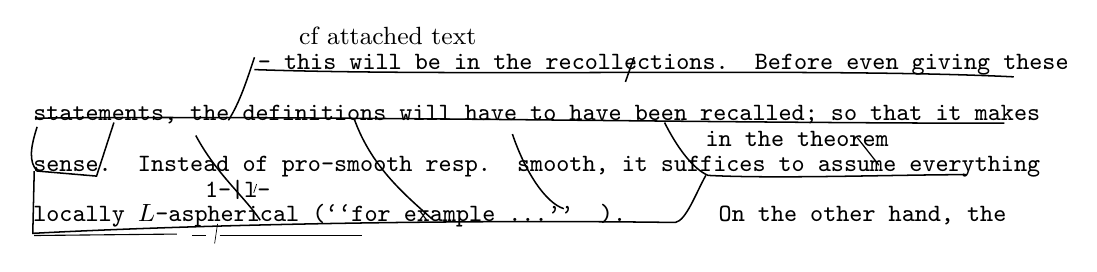
\begin{tikzpicture}[x=.0092cm,y=-.0092cm,every node/.style={inner sep=0pt,anchor=base west,font=\small\ttfamily}]
\node at (310,0) {\deleted{- this will be in the recollections\unsure{.} Before even giving these}};
\node[font=\small] at (367,-34) {\inserted{\handwritten{cf attached text}}};
\node at (0,70) {\deleted{statements, the definitions will have to have been recalled; so that it makes}};
\node at (0,140) {\deleted{sense. Instead of pro-smooth resp. smooth, it suffices to assume everything}};
\node at (928,106) {\deleted{\inserted{in the theorem}}};
\node at (237,177) {\deleted{\inserted{\unsure{1-|l-}}}};
\node at (0,210) {\deleted{\uline{locally} \uline{$L$}-\uline{aspherical} (``for example ...'' )}.};
\node at (946,210) {On the other hand, {\renewcommand{\ULthickness}{.4pt}\deleted{the}}};
\draw[line width=.55pt] (306,-17) .. controls (296,13) and (286,45) .. (270,70);
\draw[line width=.55pt] (306,0) .. controls (590,10) and (1090,-3) .. (1354,10);
\draw[line width=.55pt] (830,-17)--(818,17);
\draw[line width=.55pt] (3,67) .. controls (368,63) and (941,74) .. (1341,74);
\draw[line width=.55pt] (6,79) .. controls (-3,107) and (-6,127) .. (6,140)--(88,147)--(112,73);
\draw[line width=.55pt] (2,140)--(0,226) .. controls (247,213) and (600,207) .. (887,211) .. controls (902,208) and (915,171) .. (929,146);
\draw[line width=.55pt] (225,91) .. controls (254,145) and (293,176) .. (314,208);
\draw[line width=.55pt] (444,69) .. controls (467,132) and (509,169) .. (551,206);
\draw[line width=.55pt] (662,89) .. controls (680,142) and (708,184) .. (733,192);
\draw[line width=.55pt] (872,73) .. controls (889,107) and (911,137) .. (932,146) .. controls (1027,151) and (1191,145) .. (1289,145);
\draw[line width=.45pt] (1138,94)--(1168,132);
\draw[line width=.4pt] (2,229)--(199,227);
\draw[line width=.4pt] (220,229)--(239,229);
\draw[line width=.4pt] (258,229)--(454,229);
\draw[line width=.25pt] (309,158)--(305,170);
\draw[line width=.25pt] (255,213)--(251,240);
\end{tikzpicture}}
\endgroup
% END cancellation graphic
\reversemarginpar
\margin{\handwritten{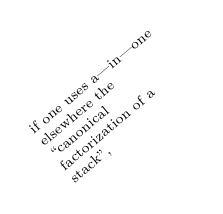
\begin{tikzpicture}[scale=.72,transform shape]
\node[rotate=40,anchor=south west,align=left,inner sep=0pt,font=\scriptsize] at (0,0) {\unsure{if one uses} \unsure{a|in|one}\\elsewhere the\\``\unsure{c}anonical\\factorization of a\\stack'',};
\end{tikzpicture}}}
\normalmarginpar
\deleted{statements} 2.12, 2.1.3, 2.1.4, 2.1.7.1 have nothing to do with schemes, they are manifestly important in themselves and should go into a separate section in
% BEGIN reference correction
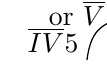
\begin{tikzpicture}[baseline=(iv.base),x=.01cm,y=.01cm]
\node[inner sep=0pt,anchor=base west] (iv) at (0,0) {\handwritten{$\overline{\text{\uline{IV}}}$}};
\node[inner sep=0pt,anchor=base west] at (47,0) {\deleted{5}};
\node[overlay,inner sep=0pt,anchor=base west] at (27,34) {\inserted{\handwritten{or $\overline{\text{\uline{V}}}$}}};
\draw[overlay,line width=.45pt] (76,-10) .. controls (81,26) and (92,36) .. (126,45) .. controls (143,51) and (150,57) .. (152,65);
\end{tikzpicture}
% END reference correction
(with a little order in the sequence of statements)

% BEGIN final cancelled line
\figure{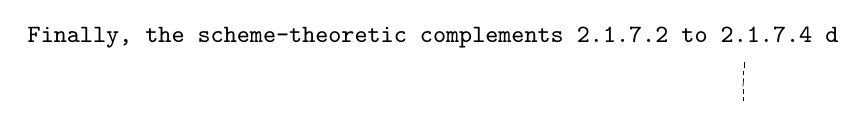
\begin{tikzpicture}[x=.0092cm,y=-.0092cm]
\node[inner sep=0pt,anchor=base west,font=\small\ttfamily] at (0,0) {\deleted{Finally, the scheme-theoretic complements 2.1.7.2 to 2.1.7.4 d}};
\draw[line width=.25pt] (990,27)--(990,34);
\draw[line width=.25pt] (989,39)--(989,45);
\draw[line width=.25pt] (989,49)--(988,60);
\draw[line width=.25pt] (988,64)--(988,70);
\draw[line width=.25pt] (988,75)--(988,80);
\end{tikzpicture}}
% END final cancelled line
% archive sheet number: 29
